\chapter{Présentation du projet}
\label{chap:Mini Projet}

\section{Le CTF}
La sécurité informatique au sein d’une entreprise est devenue le domaine avec le plus grand enjeux. Il faut donc du personnel spécialisé dans ce domaine afin de la mettre en place. On se rend facilement compte que le meilleur moyen de s’améliorer dans ce milieu est dans un premier temps de se documenter puis de réaliser des attaques. C’est à ce moment-là que le "Capture The Flag" ou bien "Capturer Le Drapeau" intervient. A l’origine, un CTF est un jeu à l’air libre où deux équipes s’affrontent pour s’emparer du drapeau de l’adversaire. On peut alors s’apercevoir que le monde informatique est semblable à celui réel. En effet, notre CTF a pour but d’infiltrer une machine cible et de trouver un document, le drapeau, en toute légalité. Le CTF s’est démocratisé en 1996 lors des premières compétitions organisées par la DEF CON. La DEF CON est la convention de hackeur la plus connue du monde. \\
Les CTF s’inspirent de la vraie vie même si cela reste un terrain d'entraînement. Les CTF reposent sur plusieurs domaines qui sont : le reverse engineering, l’exploitation web, le forensic, le réseau, la cryptographie, la sécurité mobile et la stéganographie.
Tous ces domaines sont les piliers de la sécurité informatique. Il faudra donc être polyvalent afin d’exploiter les failles et de résoudre un CTF. Nous allons donc voir au cours de ce rapports différents moyens de parvenir à nos fins.

\newpage
\section{L'organisation du projet}
A la suite du choix du projet et de la création du groupe pour ce dernier, il a fallu nous organiser afin que de communiquer de manière rapide et pratique. Nous avons donc créé un serveur Discord nous permettant de communiquer en temps réel. Discord est un logiciel gratuit de communication, réalisé pour la communauté du gaming, utilisable sur tout type de support moderne avec accès à internet. Cet utilitaire nous permet d’obtenir une banque de données, un chat vocal et textuel, le tout sur une seule application. Nous avons pu, grâce à ce support, travailler chez nous tout en travaillant ensemble.
Pour ce qui est l’écriture du rapport, nous avons choisi de travailler sur Google Drive dans le but de ne jamais perdre notre travail et aussi de l’utiliser en même temps que d’autres membres du groupe.
\\
Nous nous sommes réparti le travail et avons mis en place le diagramme de Gantt suivant afin de nous organiser :

\begin{landscape}
\begin{figure}[htp!]
\centering
  \setlength\figureheight{7cm}
  \setlength\figurewidth{9cm}
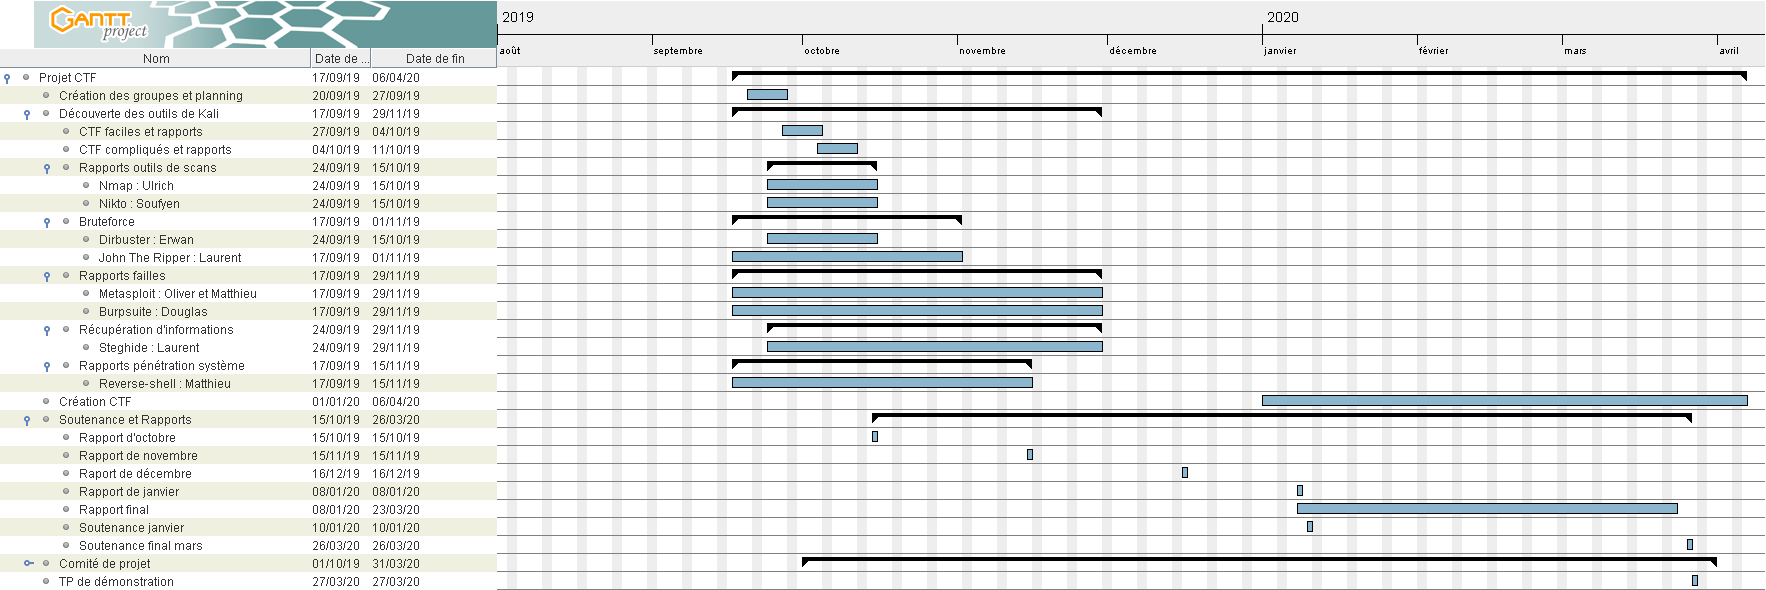
\includegraphics[height=7cm]{oui/Screens/Diag_Gantt2.png}
  \caption{Diagramme de Gantt}
  \label{fig:courbe-tikz}
\end{figure}
\end{landscape}

\section{Prise en main du projet}
Au commencement du projet, nous n’avions pas de documents fournis par les anciens élèves car nous sommes les premiers à travailler dessus. Il a donc fallu nous documenter afin de prendre en main le projet. Nous nous sommes donc tous donnés comme objectifs de réaliser des CTFs en provenance du site \textbf{Vulnhub} et d’en faire un compte-rendu pour chacun. Ces derniers sont tous stockés dans le serveur Discord afin que chacun puisse y avoir accès. Il est souvent dit que c’est en pratiquant que l’on apprend. C’est effectivement le cas ici. En réalisant les CTFs, nous avons dû nous renseigner sur les méthodes de piratage que nous allons vous détailler lors de ce rapport. Nous nous sommes servis des corrections trouvées via le site des CTFs afin de progresser et d’apprendre de nouvelles méthodes. Lorsque la correction n’était pas présente, nous avons cherché la correction de CTFs ayant des failles similaires afin de comprendre la méthode d’attaque.
Cependant, avant de vous expliquer ces méthodes, nous nous devons de vous présenter notre environnement de travail.

\subsection{Kali linux}
Kali Linux est une distribution Linux, basée sur Debian, orientée sur la sécurité informatique. Anciennement BackTrack, cette distribution a su se réinventer en devenant Kali et ainsi regrouper un nombre « incalculable » de logiciels conçus pour la sécurité et l’intrusion informatique. C’est pour cette raison que nous avons choisi de travailler sur cette distribution afin d'effectuer des CTFs.

\subsection{Mise en place d'un CTF}
Pour commencer un CTF, il nous faut aller chercher une machine virtuelle attaquable. Pour cela, nous pouvons aller sur le site de Vulnhub et récupérer un fichier avec l’extension .OVA. Ce fichier contient notre machine cible que l’on pourra allumer sous Virtualbox comme ceci :
%image importation OVA
\begin{figure}[htp!]
  \centering
  \setlength\figureheight{7cm}
  \setlength\figurewidth{9cm}
  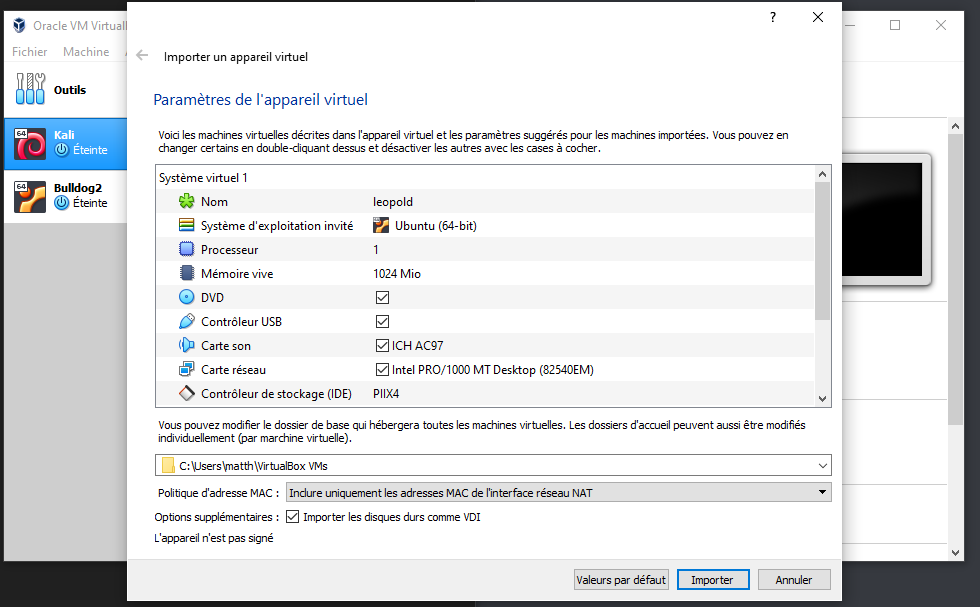
\includegraphics[width=0.7\textwidth]{oui/Screens/importation.png}
  \caption{Importation de l'OVA}
  \label{fig:courbe-tikz}
\end{figure}

\newpage
Nous conseillons de mettre en mode pont l'interface réseau de notre attaquant et de la cible. L’accès par pont est un mode d’accès réseau qui permet à une machine virtuelle d’être visible par les machines physiques du réseau. De cette manière, nos machines virtuelles pourront avoir accès au serveur DHCP du réseau et ainsi obtenir directement un adresse IP. Voici l’interface de configuration réseau de notre machine virtuelle Kali :
%image interface réseau Kali
\begin{figure}[htp!]
  \centering
  \setlength\figureheight{7cm}
  \setlength\figurewidth{9cm}
  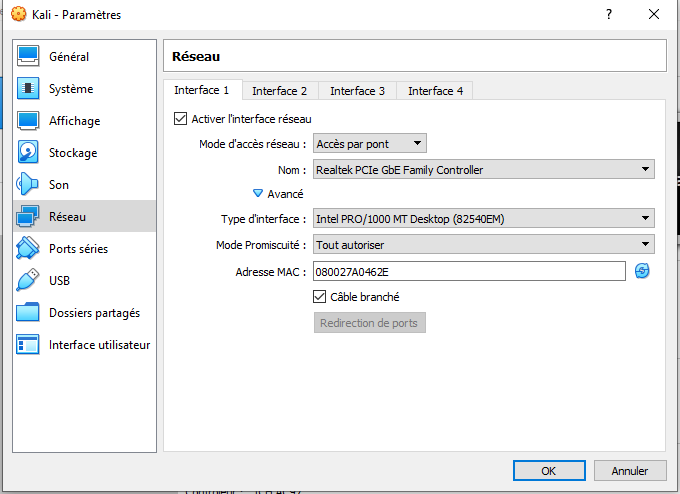
\includegraphics[width=0.7\textwidth]{oui/Screens/interface.png}
  \caption{Interface réseau de la VM}
  \label{fig:courbe-tikz}
\end{figure}

Il nous est à présent possible de commencer le CTF. \\ Voici un exemple de procédure à suivre lors de la mise en place d'une attaque Web:

\begin{figure}[htp!]
  \centering
  \setlength\figureheight{7cm}
  \setlength\figurewidth{9cm}
  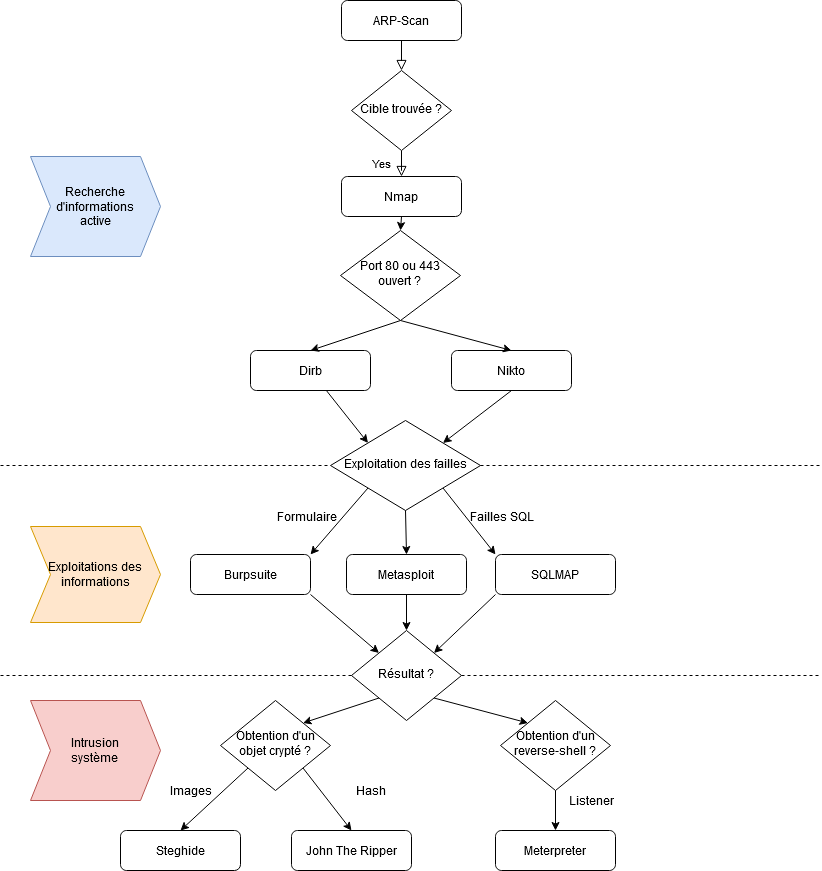
\includegraphics[width=1\textwidth]{oui/Screens/Diag/Attackdiag.png}
  \caption{Procédure d'une attaque}
  \label{fig:courbe-tikz}
\end{figure}